\chapter{Simulations} 

\section{r128} 

\subsection{drdx\_3} 

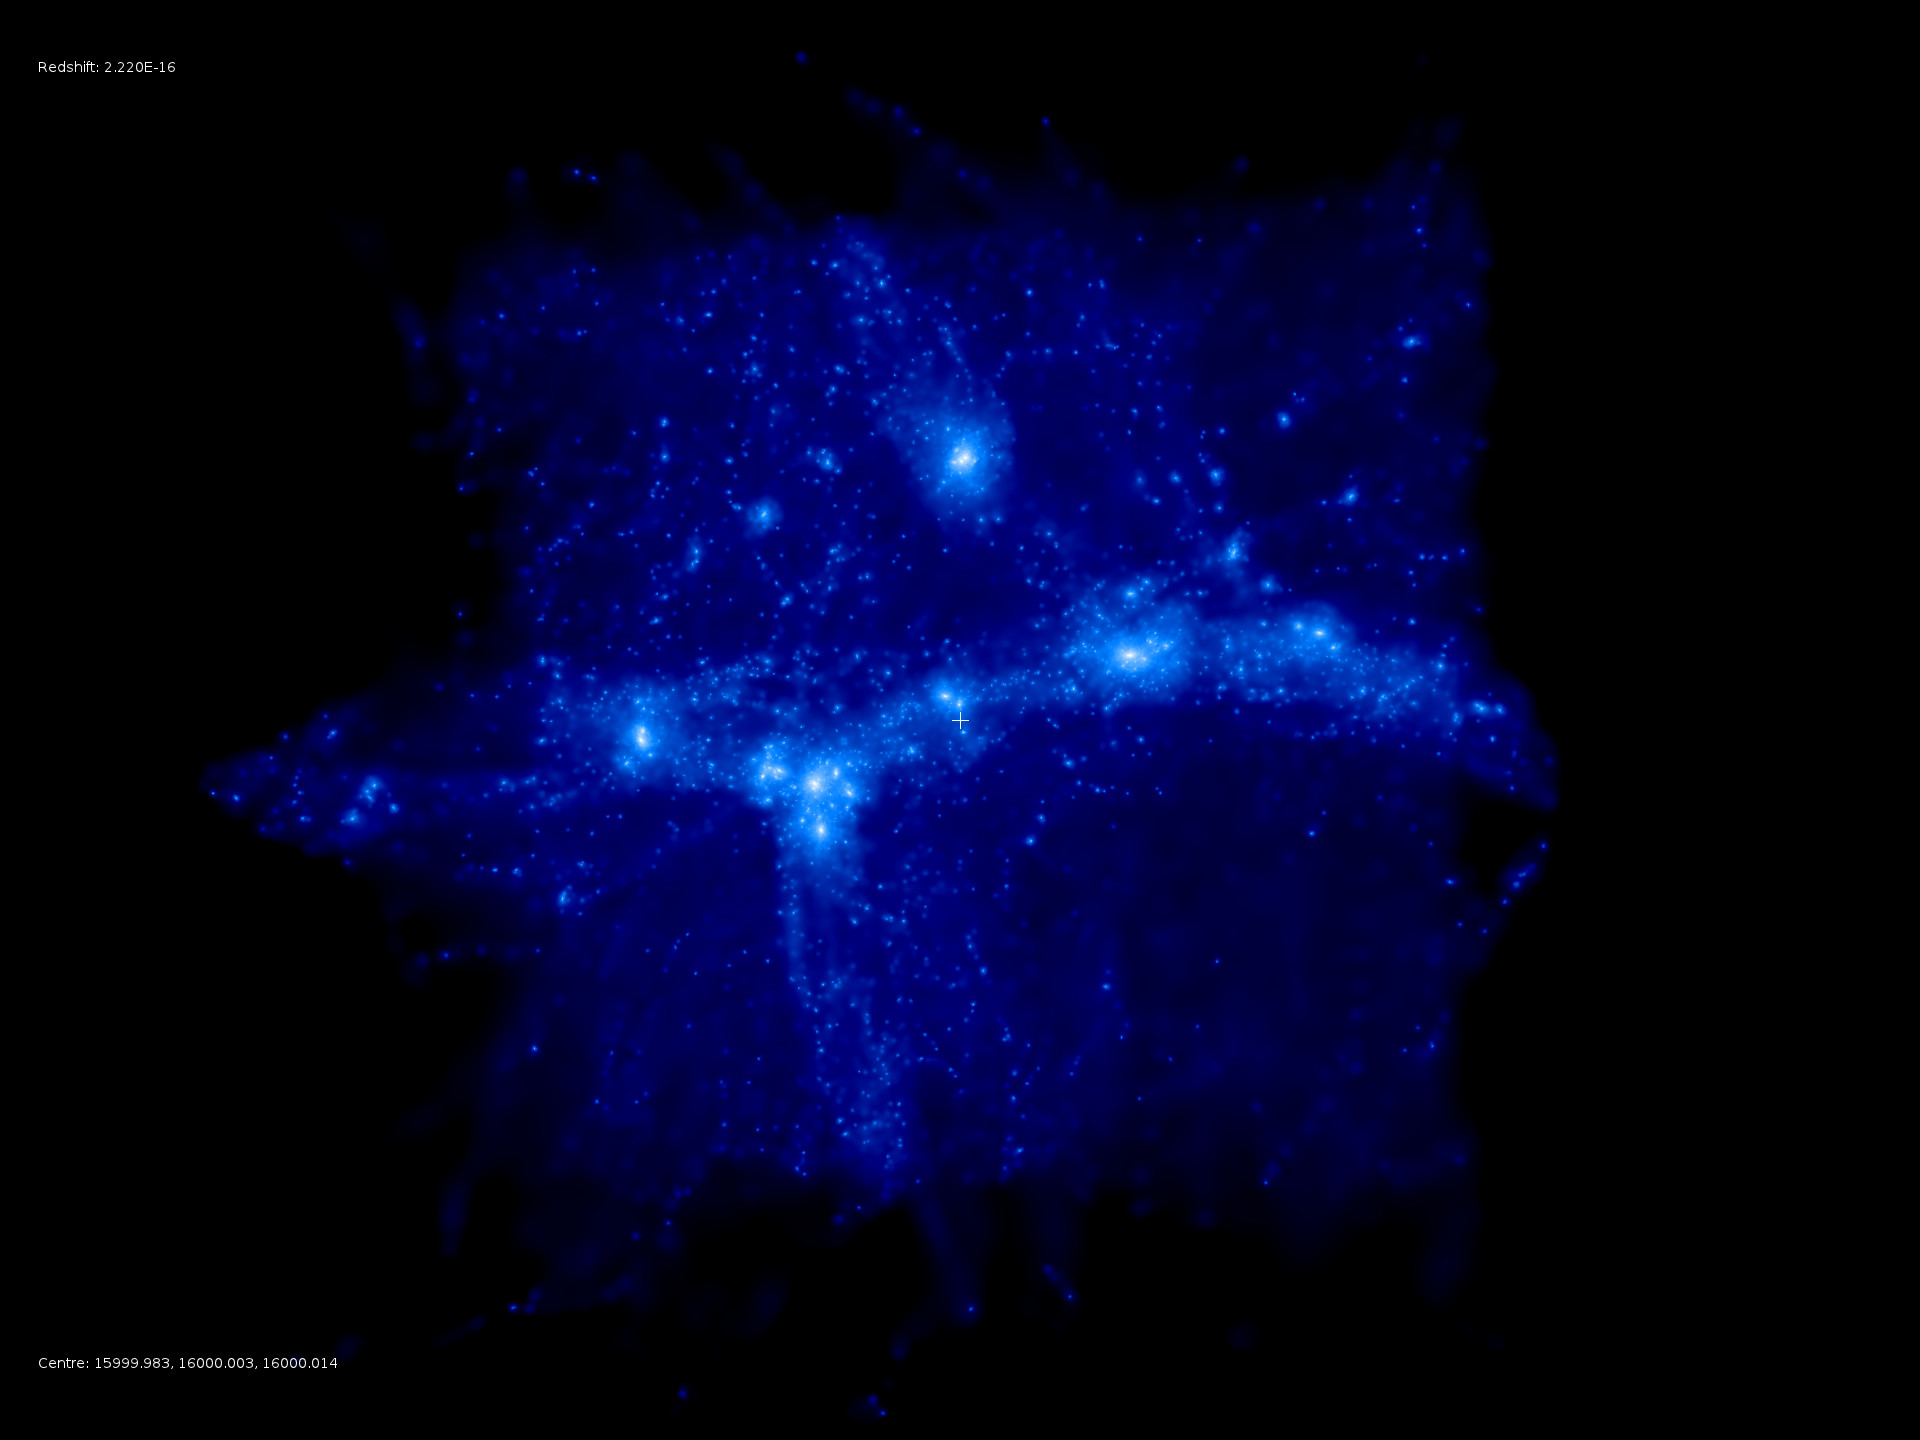
\includegraphics[scale=0.12]{drdx_3/rotate_00185.jpg} 
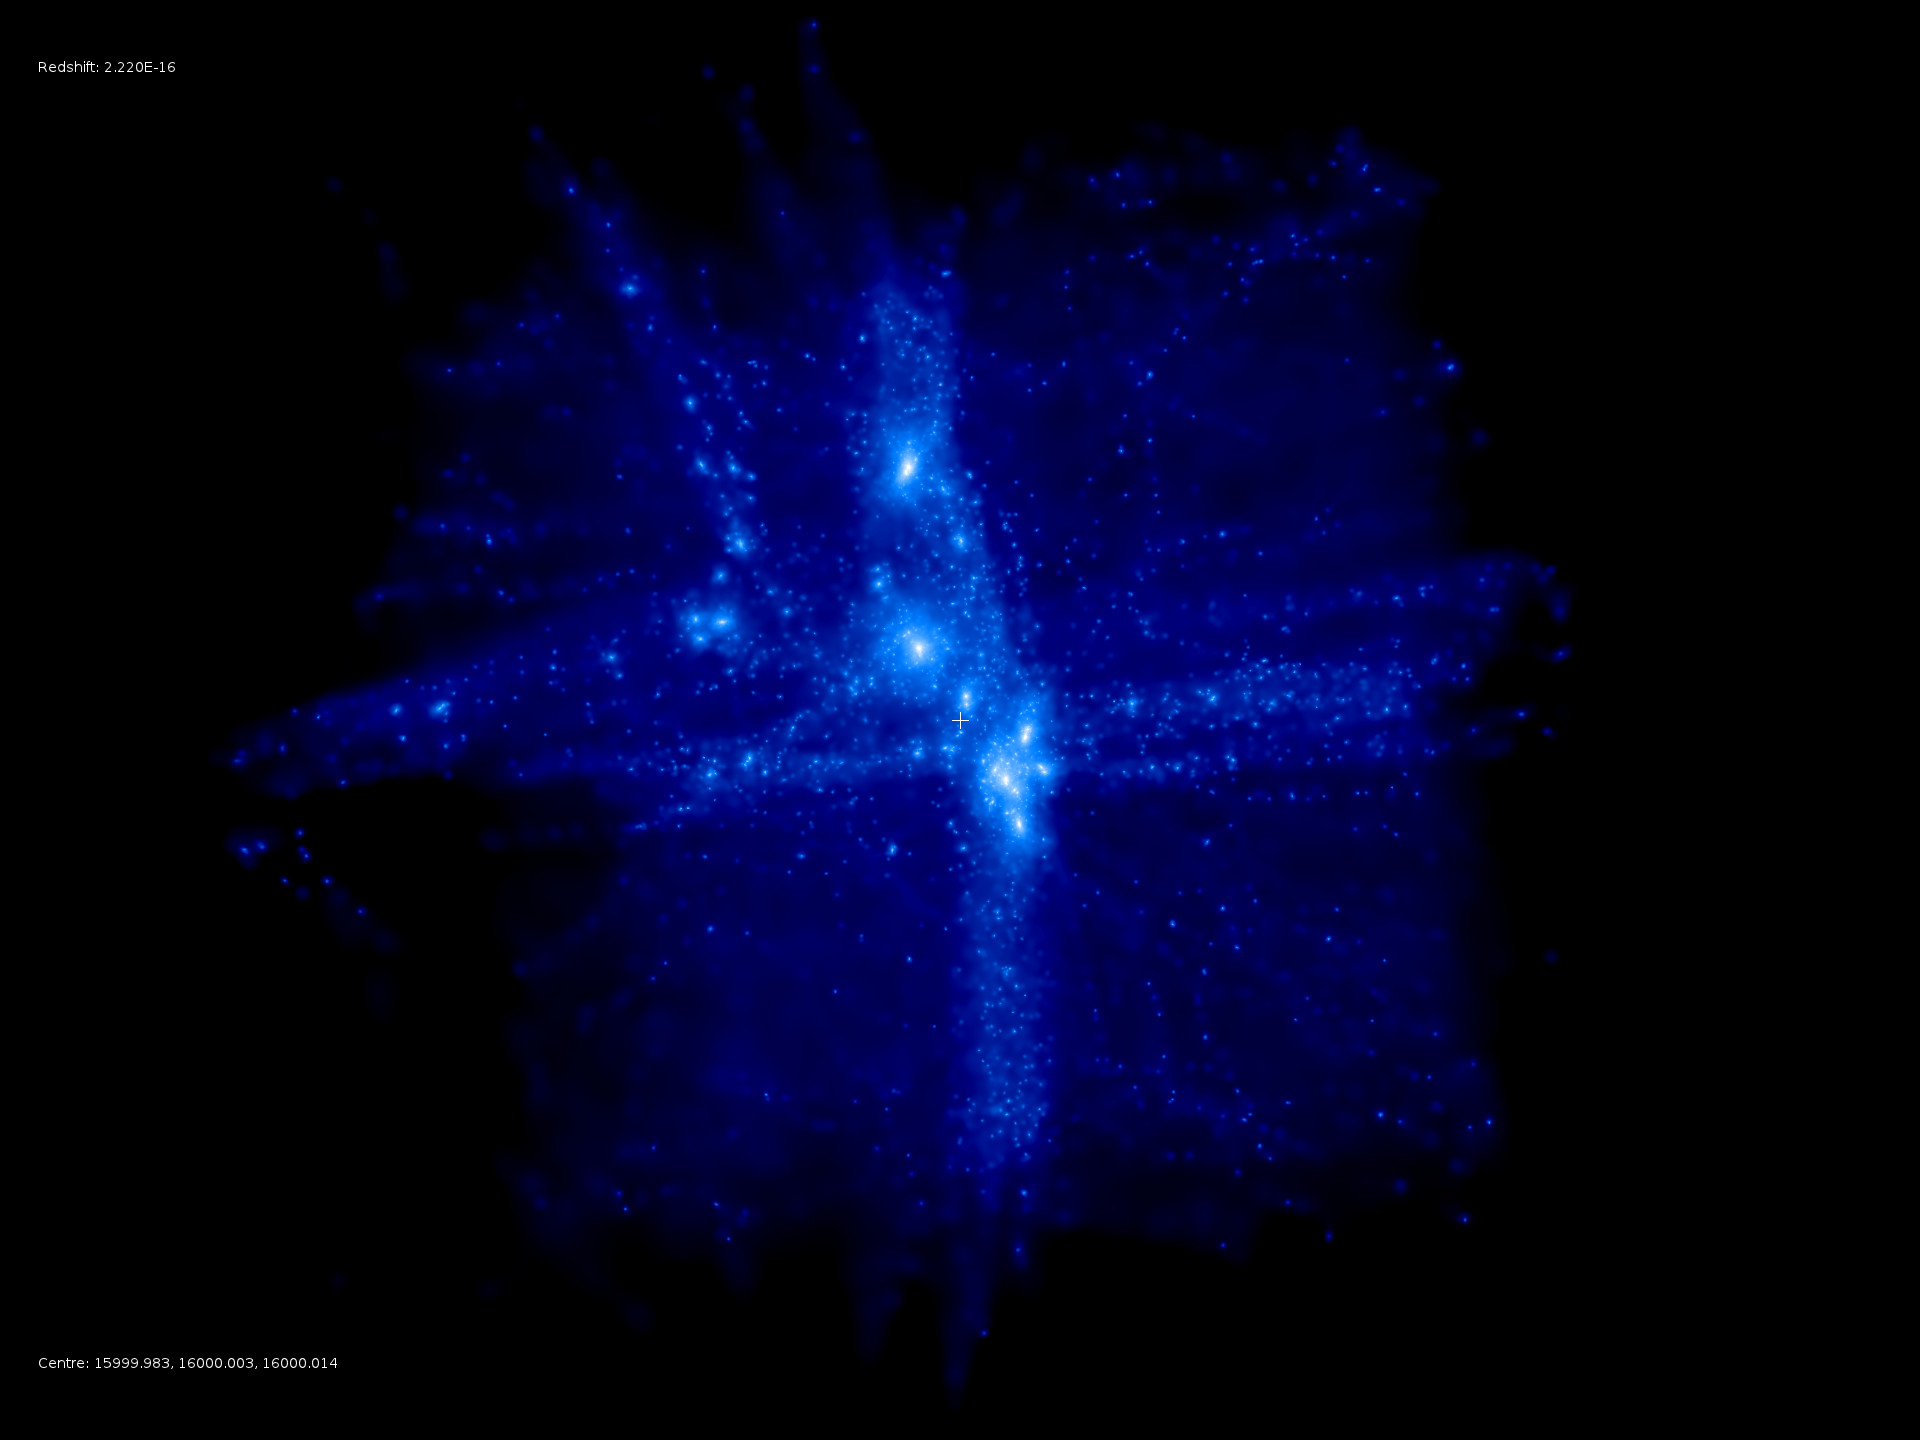
\includegraphics[scale=0.12]{drdx_3/rotate_00136.jpg} 

\textsc{rockstarred} $\surd$  \\
pfff $\rightarrow$ Error: too few halos at scale factor 0.926072 to calculate consistency metric.

\newpage
\subsection{drdx\_h100\_r128\_1}

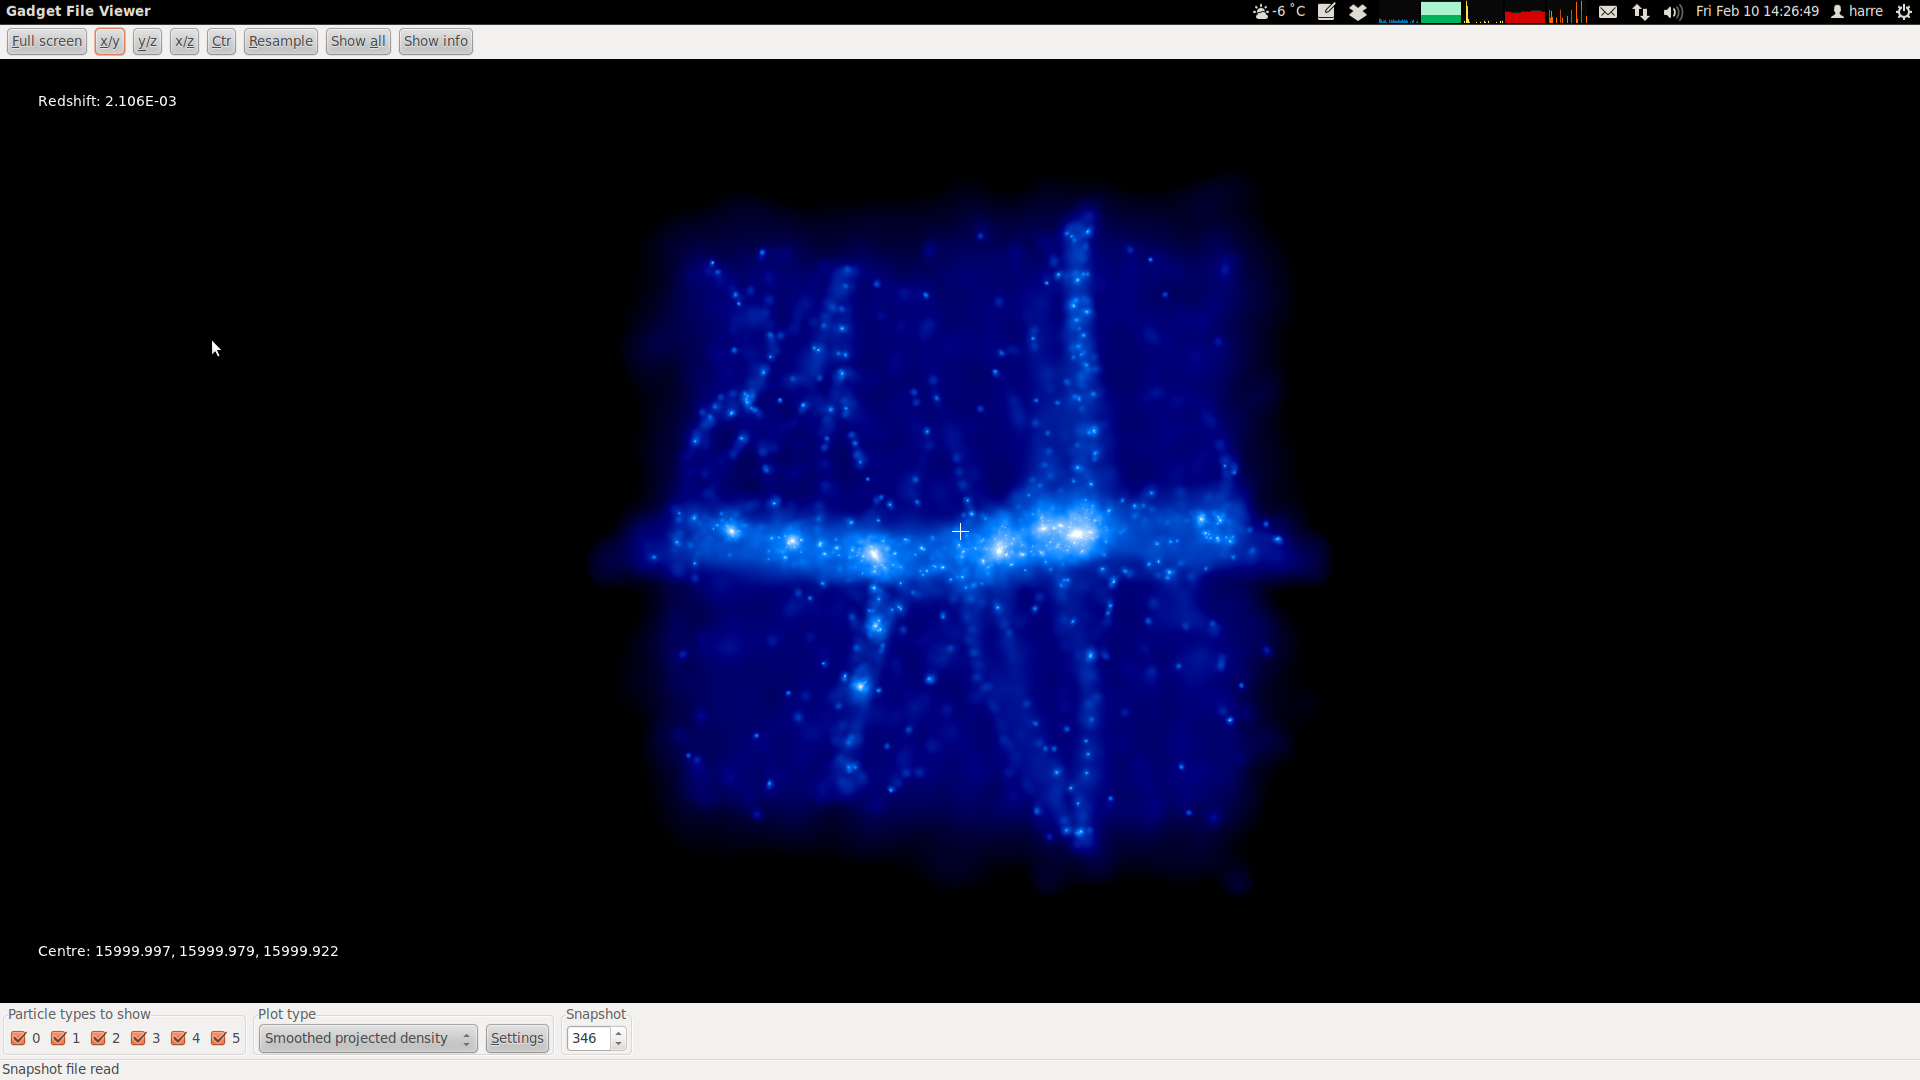
\includegraphics[scale=0.25]{drdx_h100_r128_1/1.png} 
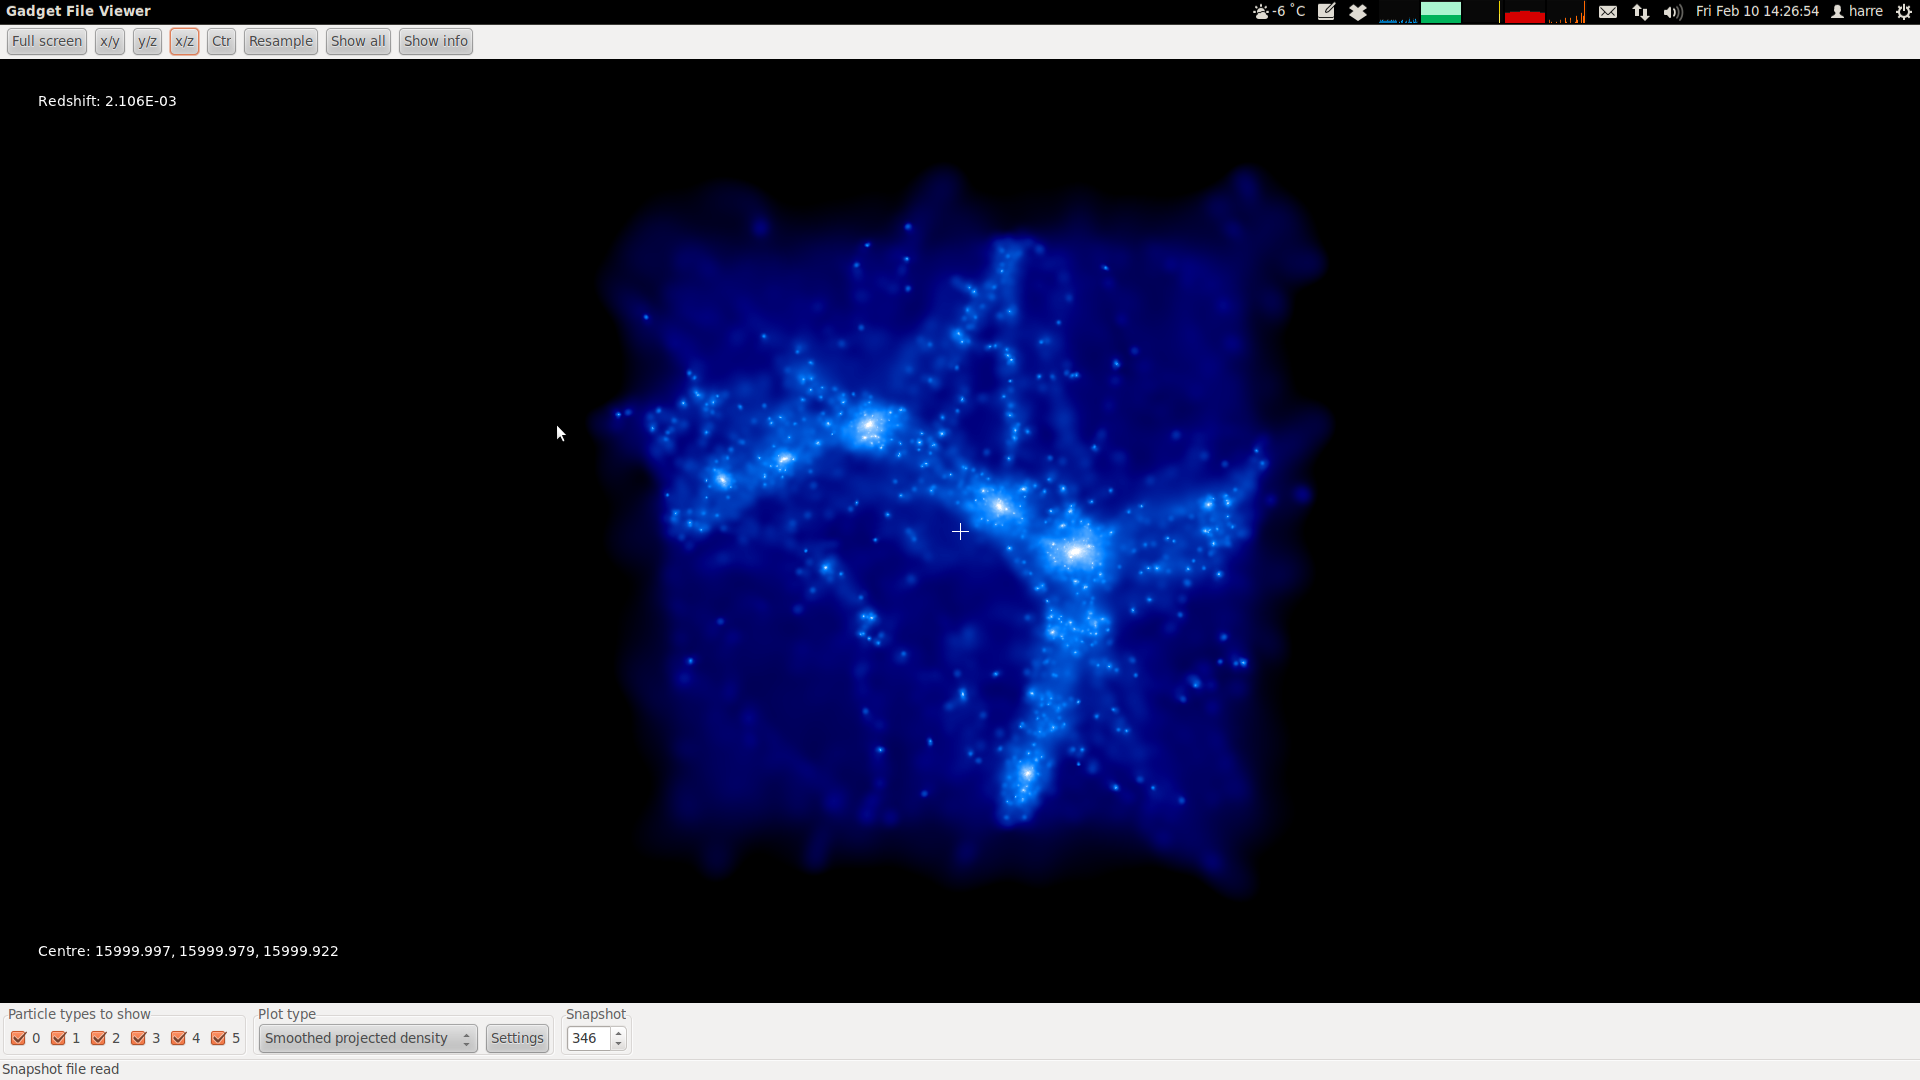
\includegraphics[scale=0.25]{drdx_h100_r128_1/2.png} 

\textsc{rockstarred} $\surd$  \\
consistenttree: too few halos at scale factor 0.896 ... $\rightarrow$ wtf? 

\newpage
\subsection{drdx\_h100\_r128\_2}

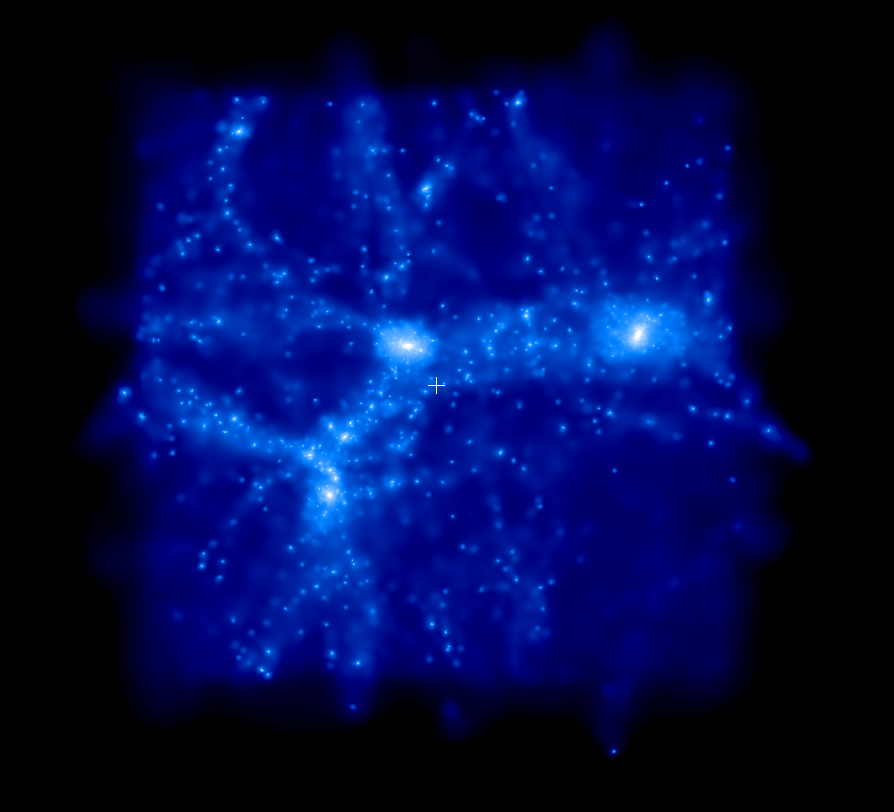
\includegraphics[scale=0.2]{drdx_h100_r128_2/1.png} 
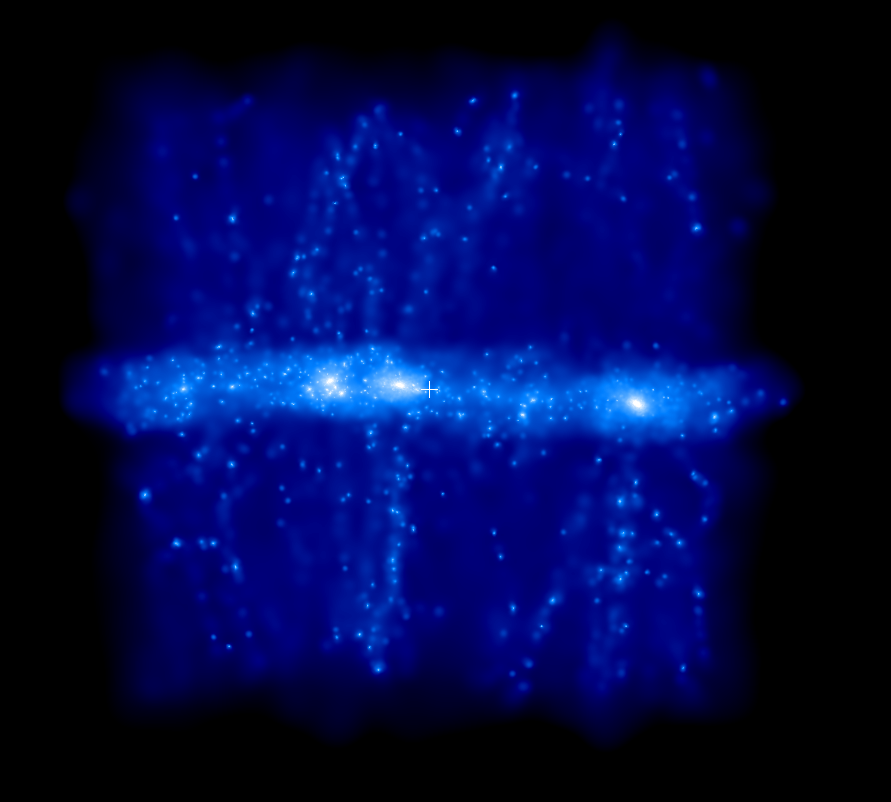
\includegraphics[scale=0.2]{drdx_h100_r128_2/2.png} 
is being rockstarred 

\newpage
\subsection{drkltest+3c+sl50\_1}
\begin{verbatim}
Error: too few halos at scale factor 0.890265 to calculate consistency metric.
Please remove this and all earlier timesteps from the scale file and rerun.
(DescScales.txt)
\end{verbatim}